\documentclass[onecolumn]{article}
%\usepackage{url}
%\usepackage{algorithmic}
\usepackage[a4paper]{geometry}
\usepackage{datetime}
\usepackage[margin=2em, font=small,labelfont=it]{caption}
\usepackage{graphicx}
\usepackage{mathpazo} % use palatino
\usepackage[scaled]{helvet} % helvetica
\usepackage{microtype}
\usepackage{amsmath}
\usepackage{subfigure}
% Letterspacing macros
\newcommand{\spacecaps}[1]{\textls[200]{\MakeUppercase{#1}}}
\newcommand{\spacesc}[1]{\textls[50]{\textsc{\MakeLowercase{#1}}}}

\title{Data Mining Final Project}
\author{Team MAD}
\date{January 2020}

\begin{document}

\maketitle

\section{Online Shoppers Intention Dataset}
\subsection{Description}
\subsubsection{Dataset}
The dataset consists of feature vectors belonging to 12,330 sessions. The dataset was formed so that each session would belong to a different user in a 1-year period to avoidany tendency to a specific campaign, special day, user profile, or period.\\

Dataset has taken from UCI Archive.

\subsubsection{Features}

Administrative: This is the number of pages of this type (administrative) that the user visited.\\
Administrative-Duration: This is the amount of time spent in this category of pages.\\
Informational: This is the number of pages of this type (informational) that the user visited.\\
Informational-Duration: This is the amount of time spent in this category of pages.\\
ProductRelated: This is the number of pages of this type (product related) that the user visited.\\
ProductRelated-Duration: This is the amount of time spent in this category of pages.\\
BounceRates: The percentage of visitors who enter the website through that page and exit without triggering any additional tasks.
ExitRates: The percentage of pageviews on the website that end at that specific page.\\
PageValues: The average value of the page averaged over the value of the target page and/or the completion of an eCommerce\\
SpecialDay: This value represents the closeness of the browsing date to special days or holidays (eg Mother's Day or Valentine's day) in\\
Month: Contains the month the pageview occurred, in string form.\\
OperatingSystems: An integer value representing the operating system that the user was on when viewing the page.\\
Browser: An integer value representing the browser that the user was using to view the page.\\
Region: An integer value representing which region the user is located in.\\
TrafficType: An integer value representing what type of traffic the user is categorized into.\\
VisitorType: A string representing whether a visitor is New Visitor, Returning Visitor, or Other.\\
Weekend: A boolean representing whether the session is on a weekend.\\
Revenue: A boolean representing whether or not the user completed the purchase.\\

\subsubsection{Researchers}
C. Okan Sakar Department of Computer Engineering, Faculty of Engineering and Natural Sciences, Bahcesehir University, 34349 Besiktas, Istanbul, Turkey\\

Yomi Kastro Inveon Information Technologies Consultancy and Trade, 34335 Istanbul, Turkey\\

\maketitle

\subsection{Our Aim on The Dataset}
\subsubsection{Explotary Data Analysis}

First of all, we want to get more information about the dataset to be more succesful for the other steps. Also, in this step will show us that is there a missing or an unnecessary data or not. Having these kind of datas prevents our models giving more accurate results.


\subsubsection{Classification}

Online Shoppers Dataset give us the some features which i show it on 1.1.2 and the item sold or not sold. So, basicly we can guess the sold or not with the features. The guessing provides us for the new sessions will buy the item or will not buy it. This can be important information for e-commerce companies with getting similar features from their costumers. For this step, we will use 3 different classification algorithms.\\

\subsubsection{Clustering}

Our other aim is clustering. We will apply pca for the features to dimension reduction to 2d or 3d. After that, we want to cluster them on plot. It show us how these customers' behavior differ.\\


\subsection{Tasks}
\subsubsection{Explotary Data Analysis(EDA)}
There was no any null-missing data in our dataset but there was same data which are effect our models in future. Our dataset problems are:\\

1. Some features are integer type which should be category type.\\
2. Some features are unnecessary to guess the revenue. For example, we dont think the browser which we use, will not help us to guess it.\\
3. There was ten different month, the data's number of six of them are insufficient.\\
4. On Administrative and Administrative Duration features includes zero value. This is really meaningless because to buy or not the item, you have to click its page. You cant buy without clicking it.\\
5. As a last, there was outliers for Durations. The customer could be click the page and could forget he/she is on page.\\



\subsubsection{Classification}
\graphicspath{ {} }
In classification step, we have choosen sgdclassifier, mlpclassifier and k-NN for classification algorithms.\\

Accuracy Scores:\\
SGDClassifier: 83.29\\
MLPClassifier: 81.47\\
k-NN: 80.12


\begin{center}
    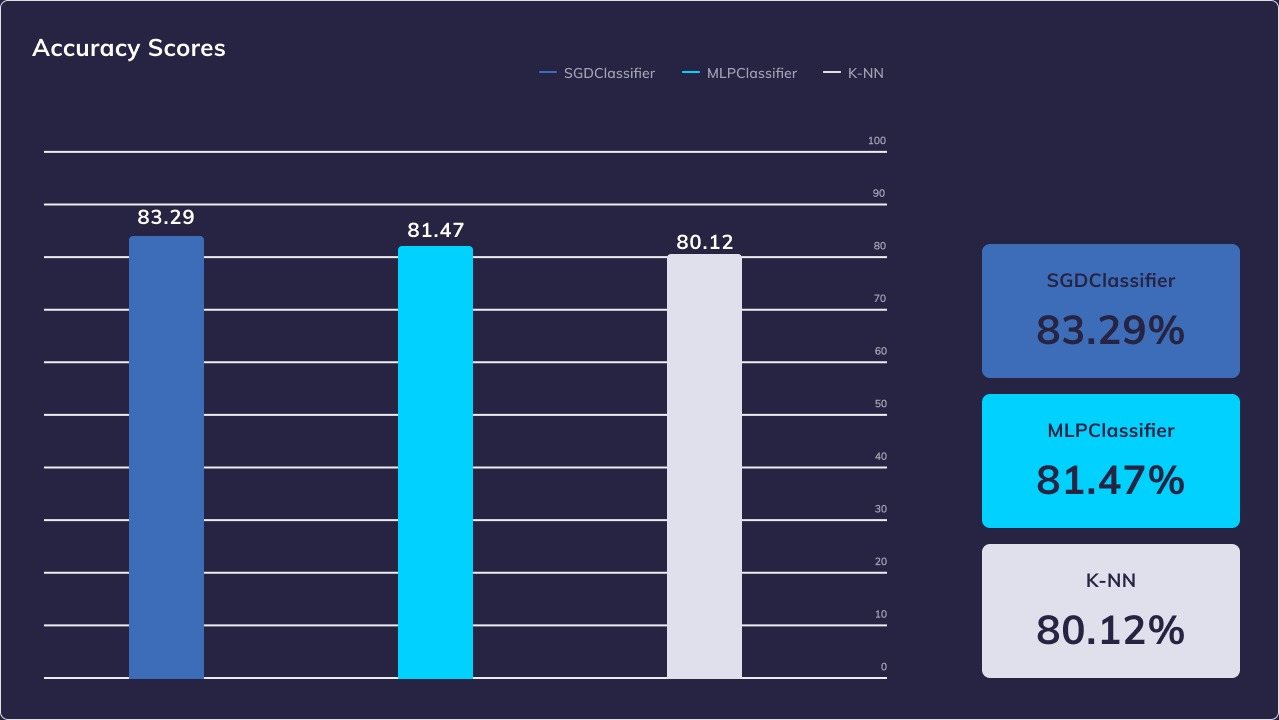
\includegraphics[width=.8\textwidth]{accuracy.jpeg}\\
    Accuracy Scores
\end{center}

\subsubsection{Clustering}

Before clustering, we've used PCA to dimension reduction to 2d looking their explained ratio. After that, We've applied K-means with Optimum K. 

\begin{center}
    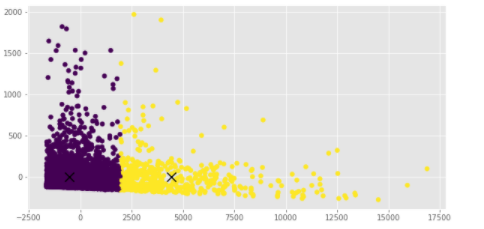
\includegraphics[width=.8\textwidth]{kmeans1.PNG}\\
    K-means with K equal to 2
\end{center}

K-means with Different K Values

\begin{center}
    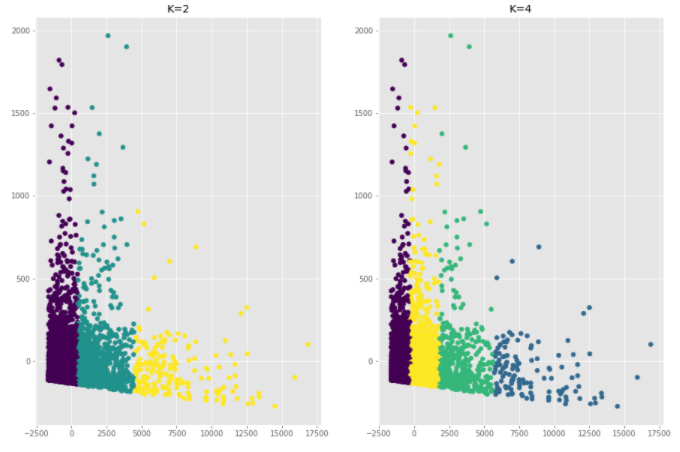
\includegraphics[width=.8\textwidth]{kmeans2.PNG}\\
    K-means with K equal to 3 and 4
\end{center}

\maketitle


\subsubsection{Chapter Conclusion}

For online shoppers intention dataset, first explotary data analysis was applied and the dataset was analyzed. Issues have been discovered and solutions founded. Before moving on to the dataset models(classification-clustering), it was first reduced and specified according to the number of observation and feature. Three different algorithms were used for classification algorithms. These were; SGDClassifier, MLPClassifier and kNN algorithms. The best score among them was obtained from SGDClassifier. For the cluster, dimension reduction with PCA was performed first. It has been made suitable for plotting. The explained variance ratios of PC1-PC2 were enough to explain the dataset. After PCA, clustering was applied with kmeans algorithm. Since optimum k is 2 according to the elbow method, it was applied with first 2 and then 3 and 4.


\end{document}